% Supplemental appendix source; not included in the six-page submission.
% The step chart requires \usepackage{tikz} when included.
\appendix
\section{Protocol Amendments}\label{app:amend}
\begin{table}[t]
\caption{Material protocol amendments. ``Pre'' means before factorial varied runs; ``post'' means after their start.}
\label{tab:amend}
\small
\begin{tabular}{@{}p{0.17\columnwidth}p{0.76\columnwidth}@{}}
\toprule
Date & Decision and inferential effect \\
\midrule
Sep. 29 & Split functional filter from timing-bound outcome; re-report original strict attrition. \\
Oct. 3 (pre) & Lock 13 tasks, three model IDs, two prompt conditions, and five repeats. \\
Oct. 4 (pre) & Replace 113-hour full RTC plan with frozen forecasts, 14-suite balanced validation sample, and all 36 nonpredictable suites; defer factorial HSI. \\
Oct. 4 (pre) & Lock shared 100-seed RTC schedule, human controls, replay, and hybrid contrast. \\
Oct. 5--7 (post) & Add source reason categories, reduced reference triage, three-fault quality arm, and static scans; these are separate descriptive or fault-injection analyses. \\
Oct. 7 (post) & Add separately registered nominal-clock $\pm1$ RTC-second alarm-programming faults with reference activation and counting controls. \\
Oct. 8 (post) & Add all-attempt, exact-test, source-similarity, internal-consistency, and upstream-pattern re-analyses; no new experiment runs. \\
\bottomrule
\end{tabular}
\end{table}

\section{Forecast Coverage and Hybrid Bounds}\label{app:hybrid}
\begin{table}[t]
\caption{Registered hybrid bounds combine measured original verdicts and frozen zero-failure forecasts for unrun predictable suites. Missing originals are bounded as passes or failures. These are not empirical confidence intervals.}
\label{tab:hybrid}
\small
\begin{tabular}{@{}llrr@{}}
\toprule
Model & Range & Eligible slots & Hybrid failures \\
\midrule
Luna & absent & 400 & 0 \\
Luna & present & 300 & 0 \\
Sol & absent & 1,500 & 24--28 \\
Sol & present & 1,500 & 0--8 \\
Astra & absent & 1,500 & 13 \\
Astra & present & 1,400 & 0 \\
\bottomrule
\end{tabular}
\end{table}

\subsection{Forecast validation}\label{app:forecast}
\begin{table}[t]
\caption{Forecast validation and measurement coverage for 66 eligible LLM-generated RTC suites.}
\label{tab:forecast}
\small
\begin{tabular}{@{}lrrl@{}}
\toprule
Category & Suites & Seed slots & Result \\
\midrule
Predictable, sampled & 14 & 1,400 & Exact vectors, 14/14 \\
Predictable, unrun & 16 & 1,600 & Forecast only: 0 failures \\
Not predictable, run & 36 & 3,600 & Measured; 12 missing \\
\bottomrule
\end{tabular}
\end{table}

For the three nontrivial sampled vectors, Sol range-absent pending r01/r03 and Astra range-absent pending r05 had predicted and observed failures of 11/11, 13/13, and 13/13 on the same 100 settings. The other 11 sampled predictable suites had 0/0 failures. Their budgets are at least 20 seconds in the frozen \texttt{forecast\_table.csv} ledger, column \texttt{budget\_seconds}, above the 18.824-second ideal slow-arrival bound. The 36 suites without a scalar prediction ran in full; source-review reasons were callback delivery/order (19), pending polling/service (15), and multistage flow (2). These reason labels were added after execution began.

\section{Detailed All-Attempt Accounting}\label{app:attempts}
\subsection{All generation attempts}
The eligible-suite results condition on surviving build, functional, and nominal gates. Table~\ref{tab:attempts} restores all five attempts in each model, prompt, and RTC task cell; the artifact's 78-cell ledger also lists every one of the 13 tasks and marks factorial HSI clock/fault results \emph{not run}. Losses are mutually exclusive: build (B), built but functionally inadequate (F), then functional but nominally failing (N). Across 90 RTC attempts, 15 failed to build, eight failed the functional gate, one failed nominally, and 66 were eligible. Confirmed clock robustness requires 100 measured passing seed verdicts with no missing outcome; the upper count additionally allows unrun zero-failure forecasts and measured zero-flip suites with missing verdicts. The stricter quality count (Q) also requires a known clock budget at most twice the legal slow-arrival bound, an explicit slow-oscillator kill, and an explicit nonarrival kill. Unknown padding and missing outcomes are not confirmed successes. Only 5/90 attempts (5.6\%) meet Q, whereas 39/90 (43.3\%) have confirmed clock robustness; those are different claims. HSI factorial variation was deferred, so no comparable HSI all-attempt clock yield exists.

\begin{table*}[t]
\caption{All five RTC generation attempts per cell. B/F/N/E are build losses, functional losses, nominal losses, and eligible suites. Clock columns are observed flips, complete passes, forecast only, and zero-flip with missing verdicts. Robust is confirmed--possible over five attempts; Q is confirmed robust, non-padded, slow- and nonarrival-killing attempts over five. Fault columns give kill counts among eligible suites for fast/slow/nonarrival oscillators and early/late alarm offsets. Offsets do not activate in counting. One Luna absent nonarrival and one Sol absent callback attempt for each offset lack verdicts; all other scored fault attempts are evaluable.}
\label{tab:attempts}
\scriptsize
\begin{tabular}{@{}lllccccc@{}}
\toprule
Model & Range & Task & B/F/N/E & Clock F/C/P/M & Robust & Q & Fault kills F/S/N/$-1$/$+1$ \\
\midrule
Luna & absent & Callback & 3/2/0/0 & 0/0/0/0 & 0--0/5 & 0/5 & 0/0/0/0/0 \\
 & & Counting & 0/1/0/4 & 0/2/2/0 & 2--4/5 & 2/5 & 0/4/3/--/-- \\
 & & Pending & 4/1/0/0 & 0/0/0/0 & 0--0/5 & 0/5 & 0/0/0/0/0 \\
Luna & present & Callback & 2/3/0/0 & 0/0/0/0 & 0--0/5 & 0/5 & 0/0/0/0/0 \\
 & & Counting & 1/1/0/3 & 0/2/1/0 & 2--3/5 & 0/5 & 0/0/3/--/-- \\
 & & Pending & 5/0/0/0 & 0/0/0/0 & 0--0/5 & 0/5 & 0/0/0/0/0 \\
Sol & absent & Callback & 0/0/0/5 & 0/4/0/1 & 4--5/5 & 0/5 & 0/5/5/4/2 \\
 & & Counting & 0/0/0/5 & 0/1/4/0 & 1--5/5 & 0/5 & 0/3/5/--/-- \\
 & & Pending & 0/0/0/5 & 2/1/0/2 & 1--3/5 & 0/5 & 0/5/5/5/5 \\
Sol & present & Callback & 0/0/0/5 & 0/2/0/3 & 2--5/5 & 0/5 & 0/3/5/5/3 \\
 & & Counting & 0/0/0/5 & 0/3/2/0 & 3--5/5 & 1/5 & 0/3/5/--/-- \\
 & & Pending & 0/0/0/5 & 0/3/0/2 & 3--5/5 & 0/5 & 0/3/5/5/5 \\
Astra & absent & Callback & 0/0/0/5 & 0/5/0/0 & 5--5/5 & 0/5 & 0/4/5/5/5 \\
 & & Counting & 0/0/0/5 & 0/1/4/0 & 1--5/5 & 0/5 & 0/0/5/--/-- \\
 & & Pending & 0/0/0/5 & 1/4/0/0 & 4--4/5 & 0/5 & 0/5/5/5/5 \\
Astra & present & Callback & 0/0/1/4 & 0/4/0/0 & 4--4/5 & 0/5 & 0/4/4/4/4 \\
 & & Counting & 0/0/0/5 & 0/2/3/0 & 2--5/5 & 2/5 & 0/5/5/--/-- \\
 & & Pending & 0/0/0/5 & 0/5/0/0 & 5--5/5 & 0/5 & 0/5/5/5/5 \\
\bottomrule
\end{tabular}
\end{table*}


\section{Between-Model Exact Tests}\label{app:betweenmodels}
Post-result, two-sided Fisher tests compare all-attempt yields within each prompt. Luna's working yield is lower than Sol's and Astra's (absent $p=0.00005$ for each; present $p=0.000011$ and $0.000116$); Sol versus Astra is non-significant in both conditions ($p=1$). For confirmed robustness, Luna versus Astra differs in both conditions ($p=0.0078$ absent; $0.0025$ present), while Luna versus Sol ($p=0.215$; $0.0502$) and Sol versus Astra ($p=0.272$; $0.450$) are non-significant at 0.05. For robust plus two kills, only present-condition Luna versus Astra ($p=0.00005$) and Sol versus Astra ($p=0.0092$) are below 0.05; absent-condition pairwise $p$ values are 0.390, 0.0502, and 0.462. Between-model observed-flip tests all give $p=1$ within either condition. Slow-fault kill comparisons are non-significant between models without ranges; with ranges, Luna versus Astra ($p=0.0015$) and Sol versus Astra ($p=0.0169$) differ, while Luna versus Sol does not ($p=0.206$). The Sol--Astra late-offset comparison is non-significant in both conditions ($p=0.211$ and $0.474$); Luna has no eligible alarm suite. The full contingency tables and exact $p$ values are retained in the analysis ledger. These exploratory tests are not multiplicity-adjusted and share only three task clusters.

\section{Paired Comparisons}\label{app:paired}
\subsection{Paired and suite-level tests}
At the suite level, any legal-clock flip occurred in 3/24 measured range-absent suites and 0/26 measured range-present suites. A two-sided Fisher exact test gives $p=0.103$, so this contrast is not significant at 0.05. Restricting to suites with all 100 verdicts gives 3/21 versus 0/21 ($p=0.232$). By task, the observed-flip counts are 0/10 versus 0/9 for callback ($p=1$), 3/10 versus 0/10 for pending ($p=0.211$), and 0/4 versus 0/7 for counting ($p=1$). Within pending, Sol has 2/5 versus 0/5 ($p=0.444$) and Astra 1/5 versus 0/5 ($p=1$); Luna has no eligible pending suite. The descriptive all-task Sol contrast is 2/11 versus 0/13 ($p=0.199$), while Astra is 1/11 versus 0/11 ($p=1$). These tests exclude forecast-only suites; the primary observed-flip analysis retains measured suites with missing seeds.

Each measured LLM suite was also paired with its matched upstream case at identical evaluable frequencies. Exact per-suite McNemar tests found 19/19 callback, 20/20 pending, and 11/11 counting suites with $p<0.05$: upstream-fail/LLM-pass discordances totaled 492, 480, and 187, respectively, and LLM-fail/upstream-pass discordances were zero. Seven callback and five pending pairs had missing LLM verdicts and were omitted. Per-suite $p$ values span $2.98\times10^{-8}$ to $5.96\times10^{-8}$ for callback, $2.98\times10^{-8}$ to $2.44\times10^{-4}$ for pending, and equal $1.53\times10^{-5}$ for counting. These are paired \emph{within-suite schedule} descriptions, not 50 independent demonstrations: suites reuse the same 100 frequencies and cluster within only three tasks. Wilson intervals elsewhere are descriptive for those sampled settings.


\section{Source Similarity}\label{app:similarity}
\subsection{Generated-to-upstream source similarity}
We compared each of the 90 generated RTC sources with its task-matched selected upstream file. A saved ledger tags every extracted \texttt{zassert} invocation as eventual occurrence (E), not-before (B), exact event calendar (X), upper bound (U), alarm-register readback (R), count/ID (C), or other. Tags may overlap; setup/API-return assertions remain \emph{other}. The rule-based tags are source cues, not a validated semantic classifier. Table~\ref{tab:similarity} reports all-attempt tag distributions; fault-profile agreement uses only the 66 eligible suites with existing probes, excluding missing and non-activating faults. The matched upstream assertion-tag vector is 65/10/0/5/50/20 in E/B/X/U/R/C order for each 15-suite model/prompt group. Higher generated exact-event tags partly reflect the frozen configured-time specification, and readback tags reflect the pending specification.

\begin{table*}[t]
\caption{RTC similarity to matched upstream source. Source metrics cover all 15 generated attempts per cell. Profile agreement is matches/evaluable fault comparisons for eligible suites only, across fast/slow oscillator, nonarrival, and applicable signed alarm offsets. Each cell with five pending suites loses five comparisons because the upstream pending early-offset original has no verdict; further missing LLM fault verdicts are excluded. API and raw-token five-gram Jaccard values are within-cell medians. Oracle entries are counts of E/B/X/U/R/C tags; an assertion can receive multiple tags.}
\label{tab:similarity}
\scriptsize
\begin{tabular}{@{}llrrrll@{}}
\toprule
Model & Range & Eligible & Profile agree & API Jaccard & Token Jaccard & Generated oracle tags E/B/X/U/R/C \\
\midrule
Luna & absent & 4 & 11/11 & 0.50 & 0.084 & 50/15/27/12/15/37 \\
Luna & present & 3 & 6/9 & 0.44 & 0.066 & 48/20/20/14/23/39 \\
Sol & absent & 15 & 50/58 & 0.36 & 0.062 & 56/21/12/8/23/37 \\
Sol & present & 15 & 46/60 & 0.38 & 0.064 & 52/24/15/11/26/40 \\
Astra & absent & 15 & 44/60 & 0.33 & 0.070 & 75/24/33/17/24/46 \\
Astra & present & 14 & 47/55 & 0.38 & 0.071 & 74/27/19/21/21/48 \\
\bottomrule
\end{tabular}
\end{table*}

API Jaccard compares statically named Zephyr calls, excluding assertions; the per-suite call sets are preserved. The token metric strips comments/whitespace and compares raw five-token shingles. Its maximum pairwise score is 0.131, so it flags no near-copy under this metric, although different file lengths and boilerplate limit that inference. Fault profiles agree often because all selected tests kill nonarrival and none kills the fast-oscillator fault; agreement alone is not evidence of equally strong oracles.


\section{Narrow HSI Arm and Upstream Scan}\label{app:hsi}
\subsection{Narrow HSI null and source scan}
The earlier registered 100-MIPS HSI arm, using a documented $\pm1\%$ HSI input range at $25\,^{\circ}$C and an integer 99/100/101-MIPS CPU approximation, observed no assertion flips in 943 upstream or 3,270 Luna evaluable seeded runs, 0/4,213 combined. It had 87 seeded startup errors and one nominal error that excluded a Luna suite. The fresh three-model factorial HSI arm was deferred. The observed legal-clock flips occur in the wide-tolerance LSI cases, not in this narrow HSI arm.

A source-only scan of 33 pinned upstream RTC, counter, and timer files marked the three selected RTC sources as clock-bound shortfalls, 23 files as needing board/API-specific bound review, and seven with no scanned pattern.


\section{Reference Timing and Upstream Patterns}\label{app:reference}
\subsection{Reference timing and upstream source patterns}
The saved reference challenges give an internal-consistency check on the simulated clock. The callback reference returns after both callbacks and records a ztest duration at the 26 sampled slow-clock frequencies where the upstream callback failed, plus both legal endpoints. Across these 28 frequencies (17--47 kHz), its saved duration minus $320000/f$ ranges from $-0.001$ to $+0.127$ seconds, with median $+0.062$ seconds. Duration includes reference setup and delivery, so it is a coarse arrival proxy rather than a direct interrupt timestamp. The callback, pending, and counting references passed all 69 distinct failing-seed challenges, all six endpoint challenges, and all three nominal controls. No reference arrival timestamp was captured at the other 74 sampled frequencies. These observations corroborate Renode's \emph{internal} clock behavior and the threshold analysis; they do not establish STM32 silicon timing or emulator fidelity to physical interrupt delivery.

The 33-file static inventory comprises 16 RTC, five counter, and 12 timer source files, including one native-simulation RTC file. Source-pattern review flags 18 with an eventual-event/count assertion, 21 with an explicit wait or window, six with polling of RTC/counter/timer state, and eight with calendar/counter readback; files can appear in several groups. Eleven mention a callback or interrupt. Counter tests sometimes check callback counts after fixed waits, which indirectly impose a delivery deadline, but none of the 33 sources explicitly measures interrupt-to-callback latency against a registered bound. One kernel-timer source allows 100 microseconds of user-thread execution latency in a remaining-time check; that is a distinct allowance. The selected callback test checks absence after three seconds and occurrence after ten more; the selected pending test checks pending state after the same windows and reads back alarm fields; the selected counting test polls calendar progress at 500-ms intervals with a finite limit. The other 30 files have different board and API contracts, so these source patterns neither prove timing adequacy nor rule out latency checks hidden in helpers or drivers.


\section{Wait Style and Padding Detail}\label{app:style}
\begin{table}[t]
\caption{LLM-generated slow-oscillator kills cross-tabulated with source wait style and clock-budget padding. All corresponding fast-oscillator kills are zero. Groups within each block partition the 66 suites.}
\label{tab:style}
\small
\begin{tabular}{@{}llr@{}}
\toprule
Source dimension & Class & Slow-clock kills \\
\midrule
Wait style & Fixed only & 39/53 \\
 & Event only & 7/9 \\
 & Fixed plus event & 3/4 \\
\midrule
Clock budget & Over-padded ($>2\times$) & 0/12 \\
 & Assessable ($\leq2\times$) & 18/18 \\
 & Not scalar-assessable & 31/36 \\
\bottomrule
\end{tabular}
\end{table}
\section{RQ4 Source Review Detail}\label{app:source}
An earlier, unblinded single-reviewer source analysis marked unjustified timing assumptions in 6/55 historical primary LLM-generated suites and 4/11 matched upstream cases, with 17 and two unknown, respectively. These sources precede the balanced factorial. In the 66 eligible factorial RTC sources, the reviewer marked 28 definite latency/ordering assumptions, 24 unknown, and 14 with no such pattern found. Among the 47 measured LLM-generated suites with zero clock-induced assertion failures, 21 had a definite latency premise, 23 were unknown, and only three had none found. For those 47, range-absent versus range-present counts were 12/21 versus 9/26 definite and 9/21 versus 14/26 unknown. These splits do not support a general claim that tolerance context substituted latency assumptions for clock assumptions. An immediate second-callback \texttt{K\_NO\_WAIT} check in a separate historical supplement is illustrative only and contributes to no factorial denominator. No dynamic delivery-latency verdict is inferred from these labels.



\section{Frozen Alarm Task Specifications}\label{app:specs}
The following text is quoted from the \texttt{Behavior to test} and \texttt{Required observable checks} fields of the frozen prompts. Both range conditions used identical task text; the range-present condition added oscillator context elsewhere in the prompt. The full prompt files are in the artifact.

\textbf{Callback task.} \emph{Behavior to test:}
\begin{quote}\small
Exercise the STM32F407 RTC alarm callbacks using the board's RTC alias. The RTC uses the independent LSI oscillator. Set calendar time to 2024-12-31 23:59:55 and alarm time to 2025-01-01 00:00:05 for both alarm channels. Use supported second, minute, and hour alarm fields (mask 7). Verify neither callback is reported prematurely, then that both are reported when the RTC reaches the alarm time. Each callback must identify its configured alarm channel.
\end{quote}
\emph{Required observable checks:}
\begin{quote}\small
Neither callback is observed before the alarm time. Both callbacks fire at the configured RTC time and report the expected alarm IDs. The test checks callbacks through observable events or protected state and applies a finite, justified bound.
\end{quote}

\textbf{Pending task.} \emph{Behavior to test:}
\begin{quote}\small
Exercise the STM32F407 RTC alarm-pending state through the board's RTC alias. Set the calendar to 2024-12-31 23:59:55 and an alarm to 2025-01-01 00:00:05. Use supported second, minute, and hour alarm fields (mask 7). Check the alarm does not become pending before the configured calendar time, then becomes pending after the RTC reaches it. No alarm callback is required.
\end{quote}
\emph{Required observable checks:}
\begin{quote}\small
The test configures and reads back a supported RTC alarm time successfully. The alarm is not observed pending before its configured RTC time. The alarm is observed pending after the RTC reaches its configured time, under a finite, justified observation bound.
\end{quote}

\section{Artifact and Reproduction Details}\label{app:artifact}
The factorial lock stores exact prompt bytes, source hashes, call order, and metadata for the 390 source-only generations. Calls used \texttt{codex-cli 0.158.0-alpha.2.1}; order was interleaved with pseudorandom seed 20261003. No backend model snapshot, sampling seed, temperature, or billed dollar amount was exposed. The RTC schedule records a separate seed-to-frequency map, simulator version Renode v1.17.0, platform, ELF, source, and trace hashes. The 100 saved settings are identical across measured suites, and both exact endpoints are separate challenges. The locked replay runner's in-memory equality flag is falsely negative because it compares a tuple with a JSON list. The reported replay agreement comes from an independent audit of persisted frequency, observation, selected case, outcome, and error fields; raw records were not changed. The invalid 1-Hz nonarrival run and its model crash are retained outside mutant scores. The separately registered alarm-offset manifest records driver, builder, source, platform, and ELF hashes, signed programming logs, selected-case verdicts, and replay traces. Initial reference attempts failed because the sandbox denied Renode history-file writes; their records remain alongside successful access-retry activation controls. Reproduction scripts and complete records are in the accompanying repository.


\section{Illustrative Figures Retained from the Long Draft}
\begin{figure}[t]
\centering
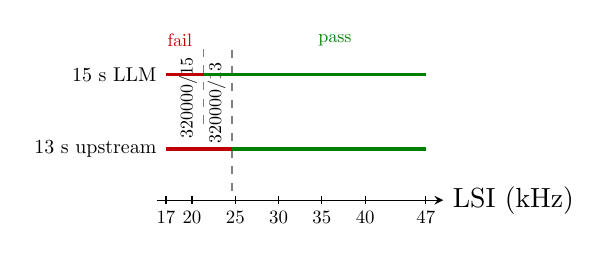
\begin{tikzpicture}[x=0.11cm,y=0.59cm,>=stealth]
\draw[->] (16,0) -- (49,0) node[right] {LSI (kHz)};
\foreach \x in {17,20,25,30,35,40,47} {\draw (\x,0.09)--(\x,-0.09) node[below,scale=.68] {\x};}
\draw[dashed,gray] (24.62,0.2)--(24.62,3.25);
\node[scale=.65,rotate=90,anchor=south] at (24.62,2.1) {$320000/13$};
\draw[very thick,red!75!black] (17,1.1)--(24.62,1.1);
\draw[very thick,green!50!black] (24.62,1.1)--(47,1.1);
\node[anchor=east,scale=.72] at (16.7,1.1) {13 s upstream};
\draw[dashed,gray] (21.33,1.65)--(21.33,3.25);
\node[scale=.65,rotate=90,anchor=south] at (21.33,2.2) {$320000/15$};
\draw[very thick,red!75!black] (17,2.7)--(21.33,2.7);
\draw[very thick,green!50!black] (21.33,2.7)--(47,2.7);
\node[anchor=east,scale=.72] at (16.7,2.7) {15 s LLM};
\node[scale=.65,red!75!black] at (18.6,3.45) {fail};
\node[scale=.65,green!50!black] at (36.5,3.45) {pass};
\end{tikzpicture}
\caption{Computed ideal-clock pass/fail steps for a 13-second upstream window and a representative 15-second LLM window. A test fails when $320000/f$ exceeds its window. The registered per-seed forecasts and observed vectors, not this schematic, determine the reported counts.}
\Description{Two horizontal frequency steps turn from failure to pass at about 24.62 and 21.33 kilohertz for upstream and representative LLM windows.}
\label{fig:step}
\end{figure}

\begin{figure*}[t]
\footnotesize
\textbf{Upstream callback, \texttt{test\_alarm\_callback.c}, lines 120, 126--127, 132, 140--141:}
\begin{verbatim}
k_sleep(K_SECONDS(RTC_TEST_ALARM_TEST_NOT_CALLED_DELAY));
zassert_equal(callback_called_mask_status_odd, 0,
              "Alarm callback called prematurely");
k_sleep(K_SECONDS(RTC_TEST_ALARM_TEST_CALLED_DELAY));
zassert_equal(callback_called_status, true,
              "Alarm %d callback should have been called", j);
\end{verbatim}
\textbf{LLM-generated Astra range-absent callback r01, \texttt{test.c}, lines 68 and 136--140:}
\begin{verbatim}
o->time_result = rtc_get_time(dev, &o->time);
zassert_true(calendar_compare(&o->time, &target) >= 0,
             "Alarm %u fired prematurely", (unsigned int)i);
zassert_equal(calendar_compare(&o->time, &target), 0,
              "Alarm %u fired outside the target RTC second",
              (unsigned int)i);
\end{verbatim}
\caption{Literal, noncontiguous source excerpts. The upstream callback oracle checks absence and then eventual arrival within a fixed window. The LLM-generated oracle checks the RTC calendar captured at callback against the requested target.}
\Description{Source excerpts show upstream absence and presence assertions around two fixed sleeps, and an LLM-generated calendar capture with early and exact-target assertions.}
\label{fig:sourcecontrast}
\end{figure*}
